The core concept was first presented for the one-dimensional 0-1 knapsack problem (KP),
leading to very successful KP algorithms.
The main idea is to reduce the original problem by only considering a set of
items for which it is hard to decide if they will occur or not in an optimal solution.
This set of items is named core.
The variables for all items outside the core are fixed to certain values.

The knapsack problem considers items $j = 1, \ldots, n$, associated profits $p_j$ and
associated weights $w_j$.
A subset of these items has to be selected and packed into a knapsack having capacity $c$.
The total profit of the items in the knapsack has to be maximized, while the
total weight is not allowed to exceed $c$.

Before defining the core of the KP it is worth to note the solution structure
of its LP-relaxation.
The LP-relaxation of an integer programming problem arises by replacing the
constraint that each variable must be integer by a constraint that allows
continuity of the variable.
The LP-relaxation of a KP is found by replacing the constraint $x_i \in \{0,1\}$
by $0 \leqslant x_i \leqslant 1$ for all $i \in \{1, \ldots, n\}$.
If the items are sorted according to decreasing efficiency values
\begin{displaymath}
  e_j = \frac{p_j}{w_j},
\end{displaymath}
it is known that the solution of the LP-relaxation consists of
three consecutive parts: the first part contains variables set to $1$, the second
pare consists of at most one split item $s$, whose corresponding LP-values is
fractional, and finally the remaining variables, which are always set to zero,
form the third part.

For most instance of KP (except those with a very special structure) the integer
optimal solution closely corresponds to this partitioning in the sense that it
contains most of the highly efficient items of the first part, some items with
medium efficiencies near the split item, and almost no items with low efficiencies
from the third part.
Items of medium efficiency constitute the core.

Balas and Zemel~\cite{balas1980algorithm} gave the following precise definition
of the core of a KP, based on the knowledge of an optimal integer solution $x^*$.
Assume that the items are sorted according to decreasing efficiencies and let
\begin{displaymath}
  a := \min\{ j | x_j^* = 0 |\}, \quad b := \max\{ j | x_j^* = 1 \}.
\end{displaymath}
The core is given by the items in the interval $C = \{a, \ldots, b\}$.
It is obvious that the split item is always part of the core, i.e., $a < s < b$.

Figure~\ref{fig:kpecore} illustrates an exact core for an hypothetical KP instance
with $13$ items.
First row represents the efficiency value $e$ of each item.
The items are sorted by descending order of efficiency.
Second row represent solution array of the LP-relaxation.
The third row represents the exact solution for the original problem.
The $8$-th item is the split item.
Notice that the split item is within the exact core.

\begin{figure}[h]
  \centering
  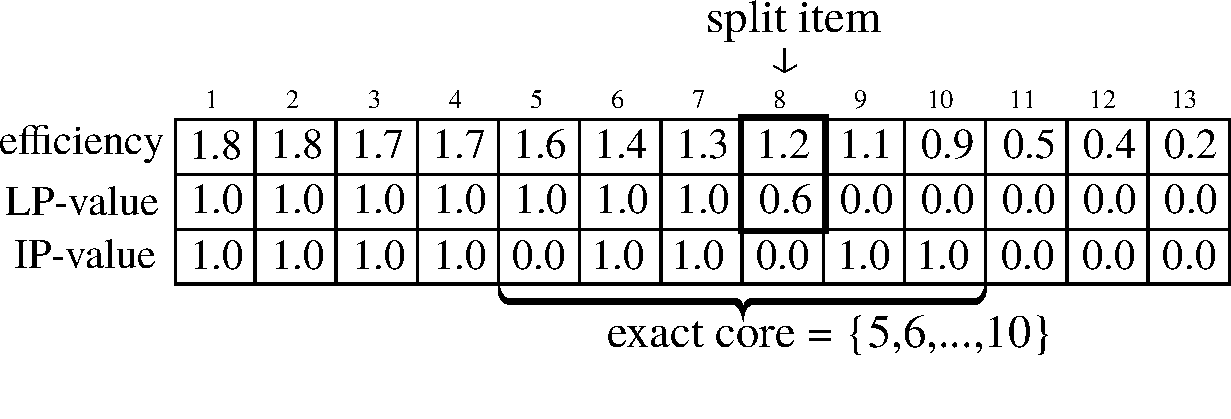
\includegraphics[scale=0.406]{imgs/core}
  \caption{Example of exact core for a hypothetical KP instance.}
  \label{fig:kpecore}
\end{figure}

The KP Core problem (KPC) is defined as
\begin{align*}
  \text{maximize} & \sum_{j \in C} p_j x_j  + \tilde{p}\\
  \text{subject to} & \sum_{j \in C} w_{j} x_j \leqslant c - \tilde{w}\\
  & x_j \in \{0, 1\}, \quad j \in C.
\end{align*}
with $\tilde{p} = \sum^{a-1}_{j=1} p_j$ and $\tilde{w} = \sum^{a-1}_{j=1} w_j$
respectively quantifying the total profit and the total weights of items fixed as selected.
The solution of KPC would suffice to compute the optimal solution of KP, which
however, has to be already partially known to determine $C$.
Nevertheless an approximate core $C = \{s-\delta, \ldots, s+\delta\}$,
of fixed size $|C| = 2\delta+1$ is considered for a heuristic reduction of the problem.

Figure~\ref{fig:kpcore} exemplifies an approximate core of a hypothetical KP
instance with $13$ items.
The first row represents the efficiency value of each item and the second row
represents the value of each variable on the LP-relaxation optimal solution.
The items are sorted in descending order of efficiency value.
The last row illustrates the variable fixing after the defined core.
Asterisks indicate free variables associated to the items in the
approximate core.

\begin{figure}[h]
  \centering
  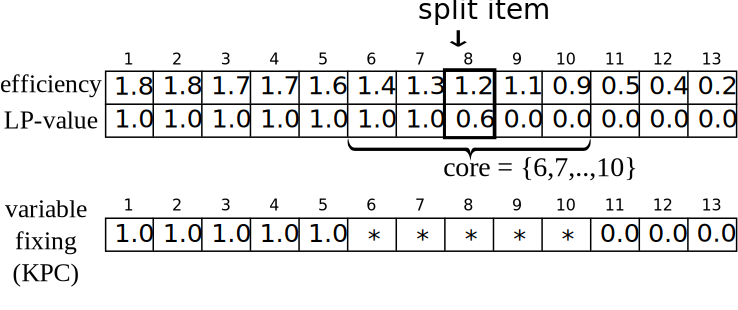
\includegraphics[scale=0.406]{imgs/kp_3}
  \caption{Example of core for a hypothetical KP instance with $n=13$ and approximate core size of $5$ ($\delta = 2$).}
  \label{fig:kpcore}
\end{figure}

\subsection{The Core Concept for MKP}

The previous definition of the core for KP can be extended to MKP without major
difficulties, once an efficiency measure is defined for the MKP,
as addressed in \cite{puchinger2006core}, even though,
a proper efficiency measure for MKP is not obvious due the
multidimensional weight of the items.
A well accepted efficiency measure is discussed in Section~\ref{subsec:dual}.

Now let $x^*$ be an optimal solution for a MKP and assume that the items are
sorted in descending order after some given efficiency measure. Then let
\begin{displaymath}
  a = \min \{ j | x_j^* = 0 \}, \quad b = \max \{ j | x_j^* = 1 \}.
\end{displaymath}
The core is given by the items in the interval $C = \{ a, \ldots, b \}$,
and the multidimensional knapsack core problem (MKPC) defined as
\begin{align*}
  \text{maximize} & \sum_{j \in C} p_j x_j  + \tilde{p}\\
  \text{subject to} & \sum_{j \in C} w_{ij} x_j \leqslant c_i - \tilde{w}_i, \quad i = 1, \ldots, m\\
  & x_j \in \{0, 1\}, \quad j \in C.
\end{align*}
with $\tilde{p} = \sum^{a-1}_{j=1} p_j$  and $\tilde{w}_i = \sum^{a-1}_{j=1} w_{ij}, i = 1, \ldots, m$.

In contrast to KP, the solution of the LP-relaxation of MKP in general does not
consists of a single fractional split item. But up to $m$ fractional values give
rise to a whole \emph{split interval} $S = \{ s_1, \ldots, s_m\}$, where
$s_1$ and $s_m$ are respectively the first and the last index of variables with
fractional values after sorting by the given efficiency measure.
Once the split interval is defined, a central index value $s = \lfloor \frac{s_1+s_m}{2}\rfloor$
can be used as the center of an approximate core.

\subsection{The Dual-variable Efficiency Measure}
\label{subsec:dual}
For defining a reasonable efficiency measure for MKP consider the most obvious
form of efficiency which is a direct generalization of the one-dimensional case:
\begin{displaymath}
	e_j(simple) = \frac{p_j}{\sum_{i=1}^{m} w_{ij}}
\end{displaymath}
In this definition different orders of magnitude of the constraints are not
considered and a single constraint may dominate the others.
This drawback can be avoided by introducing relevance values $r_i$ for every
constraint:
\begin{displaymath}
	e_j(relevance) = \frac{p_j}{\sum_{i=1}^{m} r_i w_{ij}}
\end{displaymath}
Several proposals for setting the relevance values $r_i$ were discussed and
tested by Puchinger, Raidl and Pferschy in \cite{puchinger2006core}.
According to their work setting the relevance values $r_i$ to the values of an
optimal solution to the dual problem of the MKP's LP-relaxation, as suggested
in \cite{Chu-Beasley-1998}, achieved the best results and will be the one
considered in this work for the development of the hybrid heuristic.

While the original MKP can be seen as a resource allocation problem,
the dual problem of the MKP can be seen as a resource valuation problem.
For this reason the values of the dual solution is related to the
\emph{importance} of each resource.

The split interval resulting from the efficient measure considered can be
precisely characterized.
Let $x^{LP}$ be the optimal solution of the LP-relaxation of MKP.
Then the following relation holds, as proved in \cite{puchinger2006core}:
\begin{displaymath}
 x_l^{LP} =
  \begin{cases}
    1         & \mbox{if } e_j > 1, \\
    \in [0,1] & \mbox{if } e_j = 1, \\
    0         & \mbox{if } e_j < 1.
  \end{cases}
\end{displaymath}
From this relation we can note that all variables in the split interval will
have efficiency measure $e_j = 1$, while less and more efficient ones will have
$e_j < 1$ and $e_j > 1$ respectively.

Figure~\ref{fig:mkpcore} exemplifies an approximate core of a hypothetical MKP
with $13$ variables and $3$ dimensions.
Notice that the LP-relaxation solution has now $3$ fractional variables that
defines the center of the split interval.

\begin{figure}[h]
  \centering
  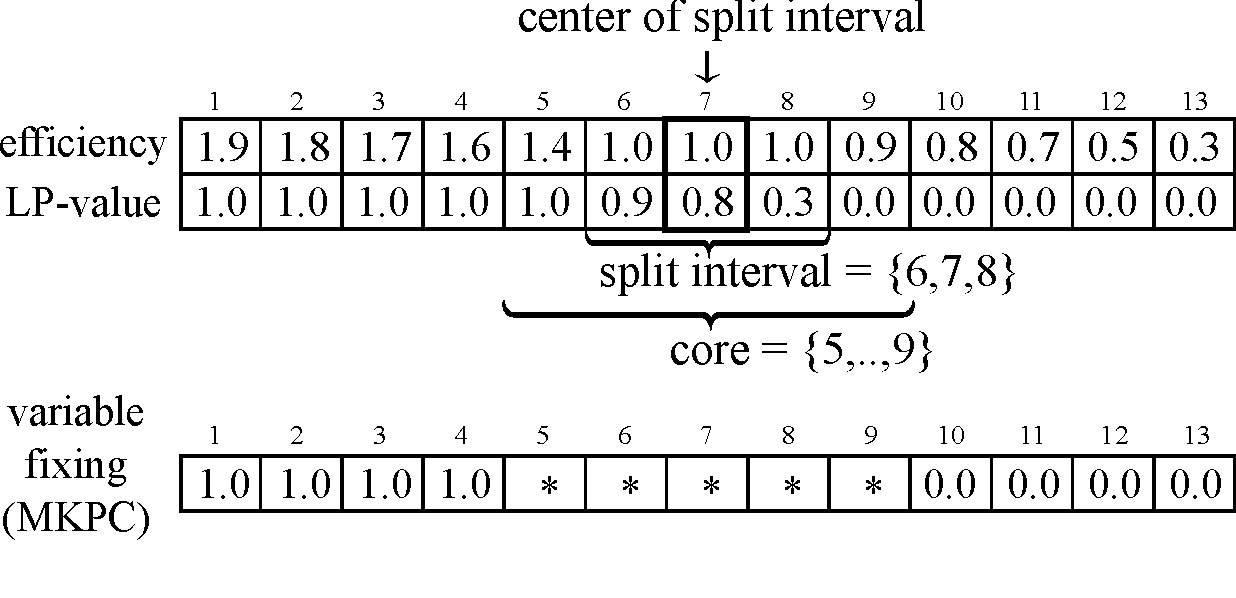
\includegraphics[scale=0.406]{imgs/mkp_3}
  \caption{Example of core for a hypothetical MKP instance with $n=13$, $m=3$ and approximate core size of $5$ ($\delta = 2$).}
  \label{fig:mkpcore}
\end{figure}

The following section presents the shuffled complex evolution algorithm
and proposes its application on the MKP.
